\documentclass[11pt]{article}

% Language setting
% Replace `english' with e.g. `spanish' to change the document language
\usepackage[french]{babel}

% Set page size and margins
% Replace `letterpaper' with `a4paper' for UK/EU standard size
\usepackage[letterpaper,top=2cm,bottom=2cm,left=3cm,right=3cm,marginparwidth=1.75cm]{geometry}

% Useful packages
\usepackage{amsmath}
\usepackage{graphicx}
\usepackage[colorlinks=true, allcolors=blue]{hyperref}
\usepackage{subcaption}
\usepackage{float}


\begin{document}

\begin{titlepage}
\title{Projet mécanique céleste "Orbital"}
\author{Bellana Carme et Romain Loustalet Palengat}

\end{titlepage}
\maketitle
\vspace{1cm}
\begin{center}
{\Large\itshape Remerciements à Monsieur Franck Rabilloud pour ses conseils et sa présence tout au long du projet, son implication dans notre apprentissage et la qualité de ses cours. Remerciements à tous nos camarades avec qui nous avons échangé régulièrement, bienveillance et partage nous ont permis de progresser dans les moments difficiles du projet. \par}
\vspace{2cm}
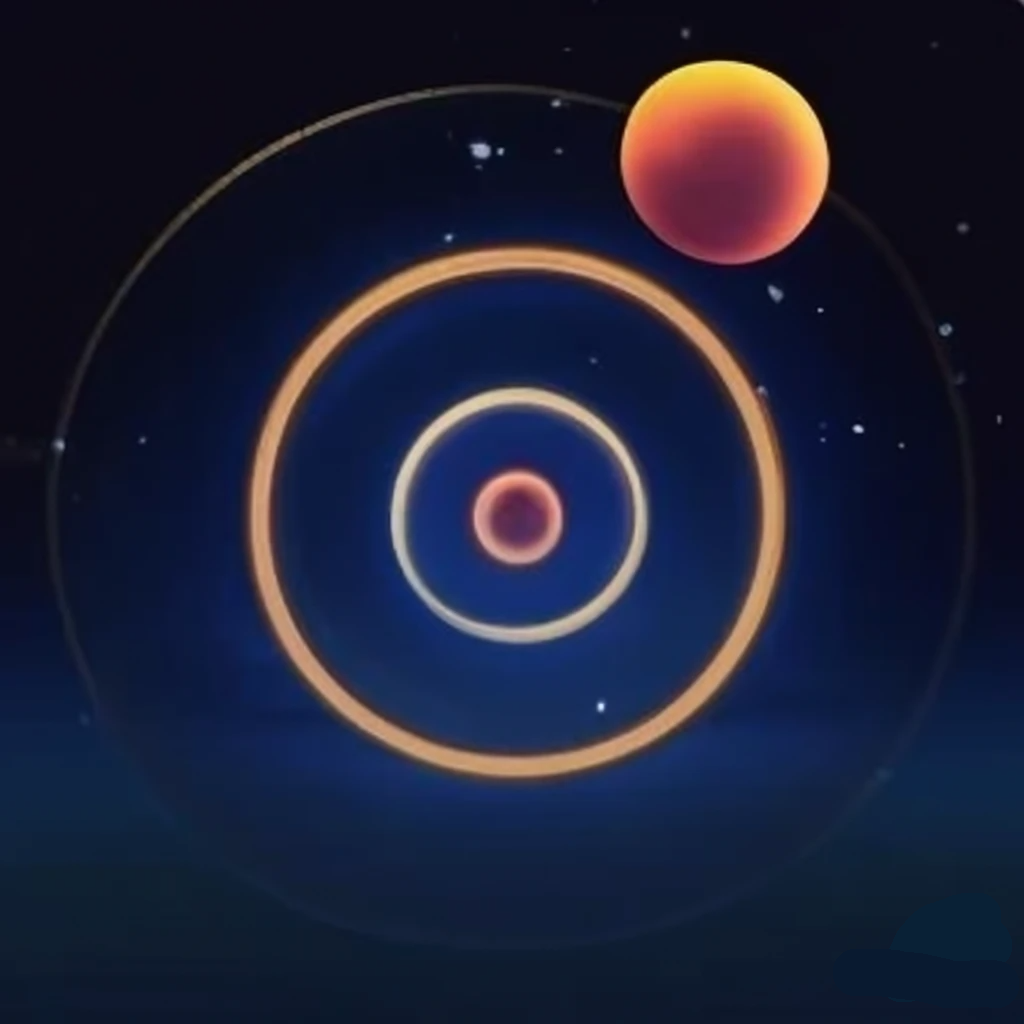
\includegraphics[width=0.4\textwidth]{logo_orbital.png}

\vfill
\end{center}
\newpage

\tableofcontents

\section{Introduction, contexte et objectifs}

Dans le cadre de l'UE Modélisation Numérique du Master de Physique Fondamentale et Applications, notre groupe, composé de Bellana Carme et Romain Loustalet Palanget, a choisi comme sujet la Mécanique Céleste.\\

Nous avons opté pour ce sujet en raison de notre ambition commune de travailler dans le domaine de l'astrophysique et de la cosmologie observationnelle, où la manipulation de programmes de modélisation est indispensable, voire la création de tels programmes. Ainsi, réaliser un projet numérique dans ce domaine nous semblait pertinent et stimulant.\\

L'objectif de notre projet est d'appliquer nos connaissances en physique et en programmation C++ pour simuler le mouvement des corps célestes au sein de leur système stellaire. Pour ce faire, nous allons intégrer les équations du mouvement en utilisant des méthodes de résolution numérique des équations différentielles.\\

\section{Méthodes utilisées}
\subsection{Organisation}

Nous avons entamé notre projet par une discussion sur nos objectifs et la manière d'y parvenir. Nous avons convenu que la programmation orientée objet serait un choix judicieux pour garantir la facilité et la clarté d'utilisation de nos programmes. En outre, nous avons mis en place différents outils de gestion de projet pour rendre celui-ci plus accessible, tels qu'un diagramme UML pour la partie programmation et un dépôt GitHub pour le versionnage de notre programme.

\begin{center}
\begin{figure}
    \centering
    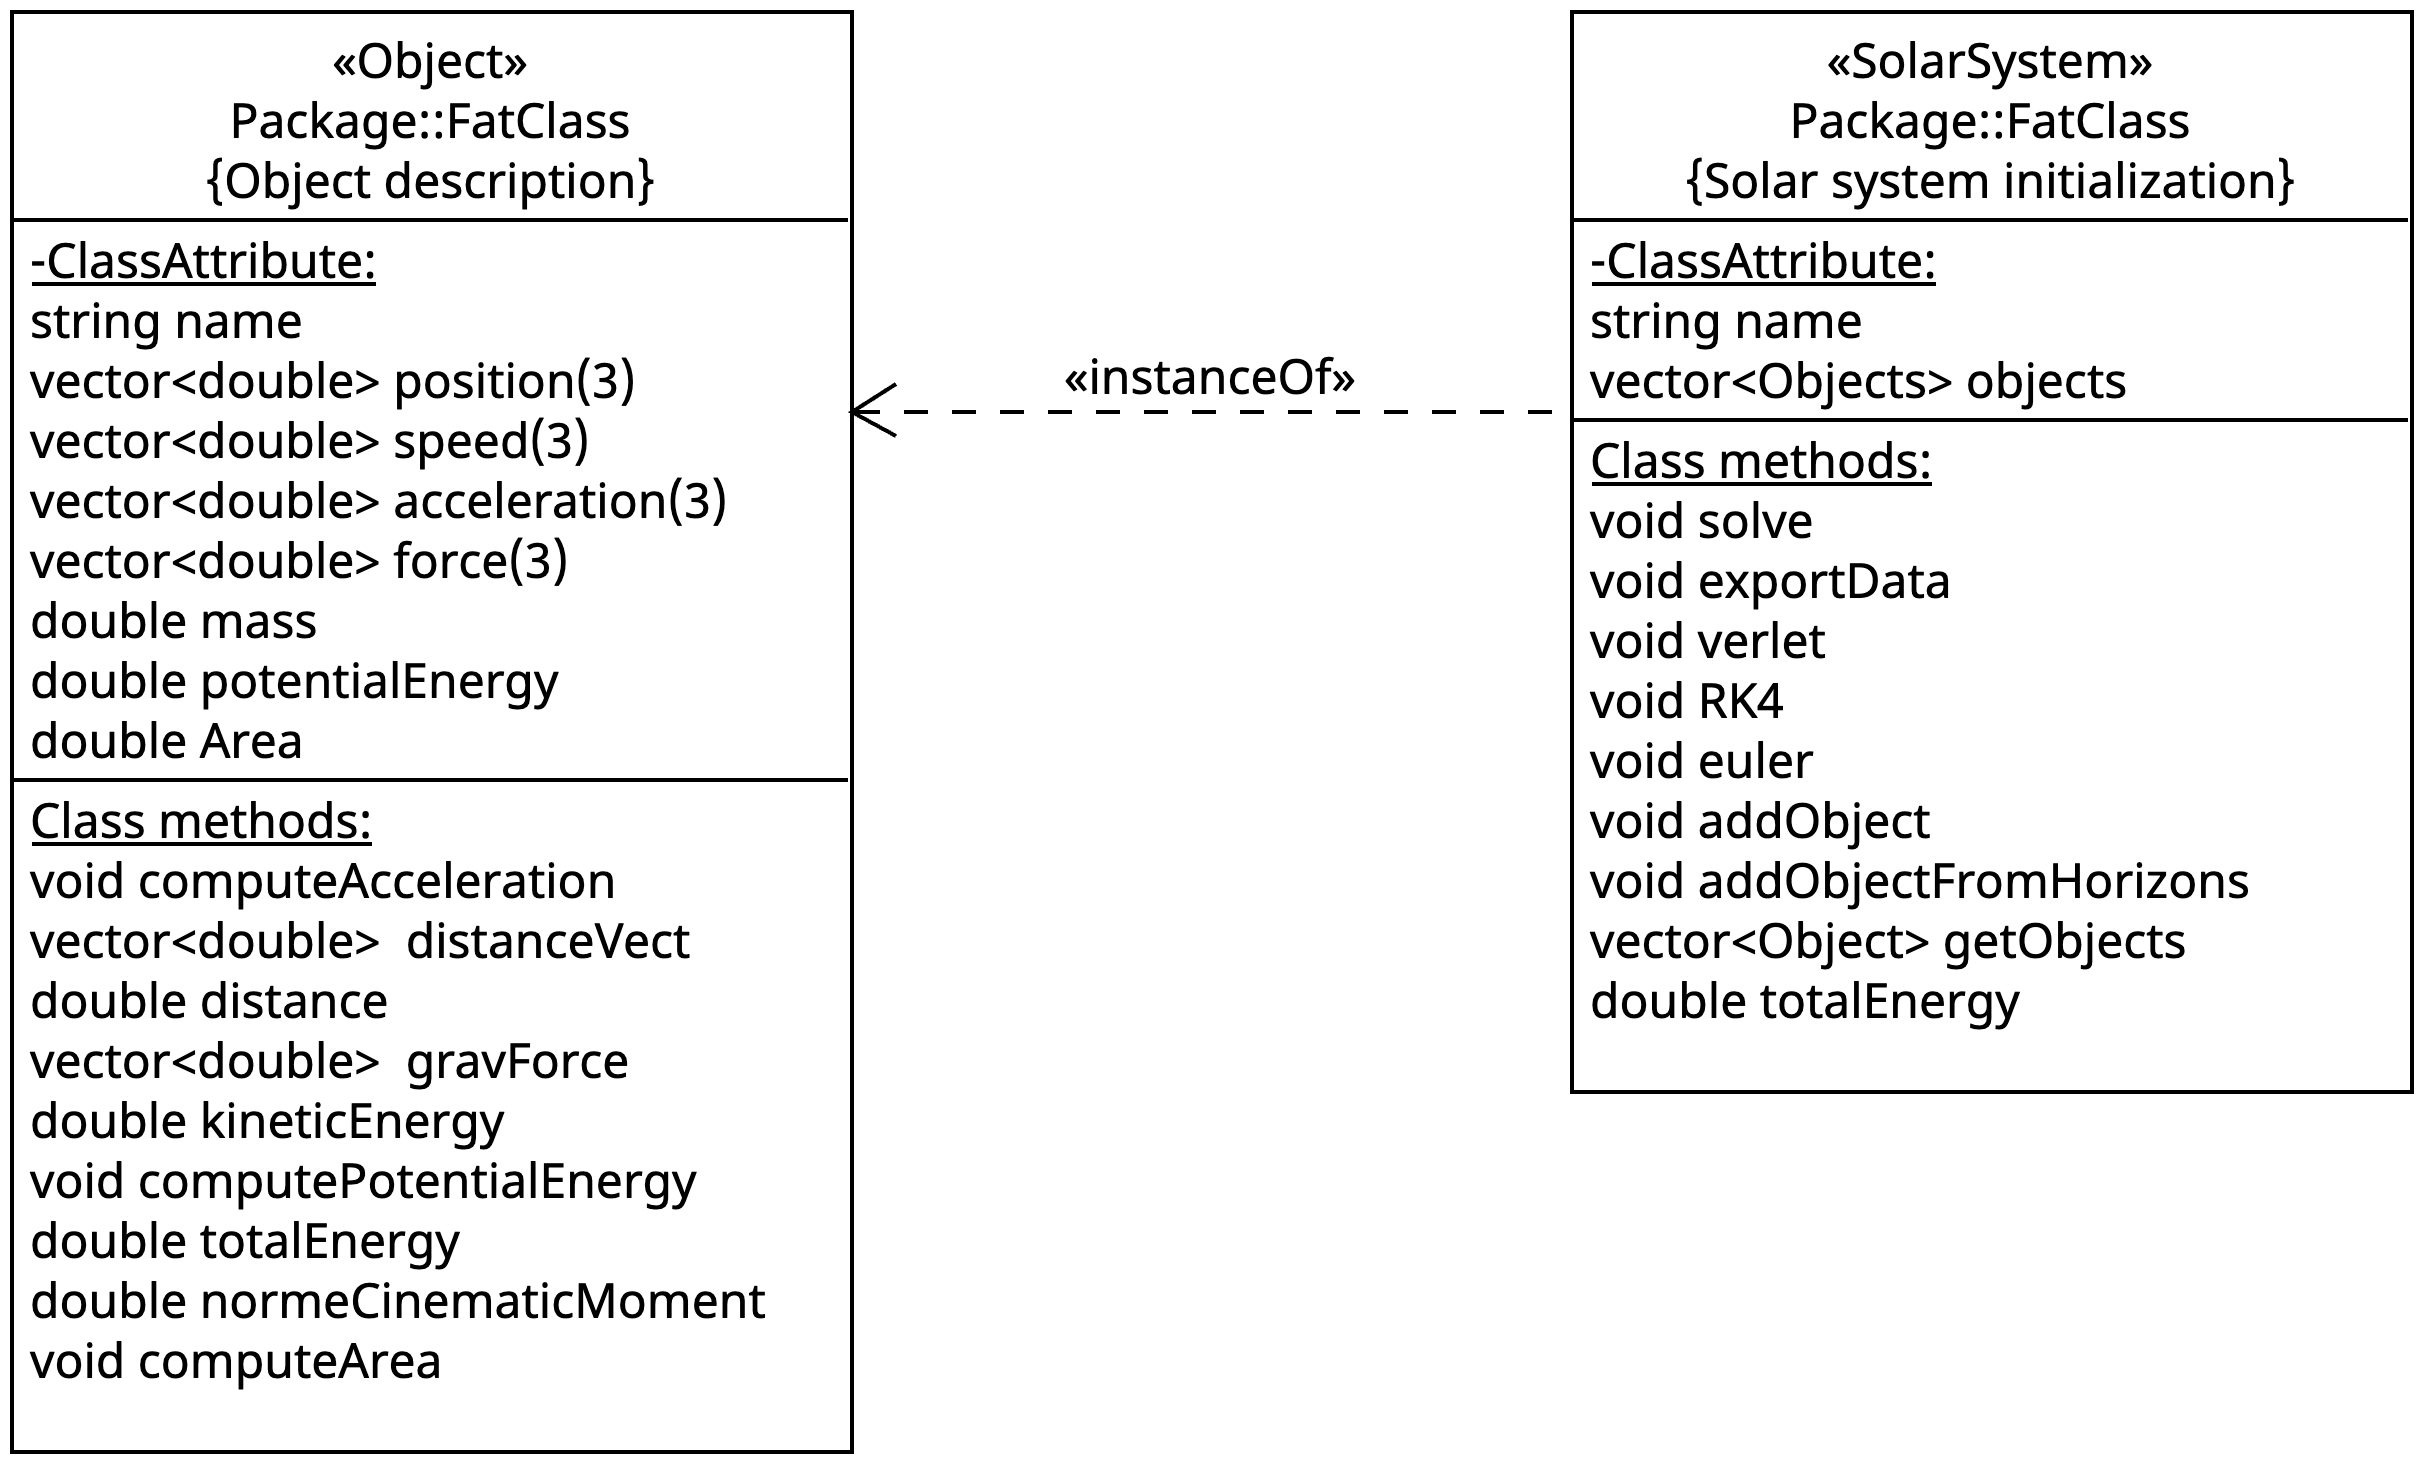
\includegraphics[width=0.7\linewidth]{orbial.png}
    \caption{Diagramme UML}
    \label{Diagramme UML}
\end{figure}
\end{center}
\subsection{Calcules physiques}

Dans le cadre de la modélisation d'un système stellaire, il est crucial de déterminer quelle force agit sur chaque objet. La force principale (et la seule que nous allons prendre en compte) est la force de gravitation. Cette force est calculée entre deux objets et dépend de leur masse ainsi que de la distance qui les sépare. Puisque chaque objet constituant le système possède une masse, il est nécessaire de calculer la force appliquée sur un objet en prenant en compte la somme des forces exercées par tous les objets environnants. Dans cette optique, nous avons utilisé la mécanique newtonienne pour déterminer la position des objets considérés à un instant donné.
\\[2 mm]
Nous partons dans un premier temps de la force gravitationnelle qu'un corps i exerce sur un corps j.
\\[2 mm]
\begin{equation}
\overrightarrow{F}_{i\overrightarrow{}j} = - \frac{G m_{i}m_{j}}{{||\overrightarrow{r_{j}}-\overrightarrow{r_{i}}||}^3}{(\overrightarrow{r_{j}}-\overrightarrow{r_{i}})}
\end{equation}
\\[2 mm]
Il faut généraliser cette équation à N corps, car on va calculer pour chaque objet i du système l'impact gravitationnel que tous les autres objets N-1 ont sur l'objet i pour chacune des composantes spatiale. On a donc pour j allant de 1 à N. De la force on va pourvoir déduire l'accélération :
\\[2 mm]
\begin{equation}
\overrightarrow{a}_{i} =\frac{\sum^{N}_{j=1,j \neq i}\overrightarrow{F}_{i\overrightarrow{}{j}}}{m_{i}}
\end{equation}
\\[2 mm]
De l'accélération, on intègre pour avoir la vitesse : \(\overrightarrow{v_{i,0}}\) est la vitesse initial de l'objet i (ou au temps précédent dans le cas d'une méthode itérative).
\\[2 mm]
\begin{equation}
\overrightarrow{v}_{i} = \overrightarrow{a}_{i}*t + \overrightarrow{v_{i,0}}
\end{equation}
\\[2 mm]
Et pour finir, on intègre la vitesse pour avoir la position \(\overrightarrow{d_{i}}\), ici \(\overrightarrow{d_{i,0}}\) est la position initiale de l
\\[2 mm]
\begin{equation}
\overrightarrow{d}_{i} = \frac{\overrightarrow{a}_{i}*t^{2}}{2} + v_{i,0}*t + \overrightarrow{d_{i,0}}
\end{equation}
\\[2 mm]



Ensuite on a les différentes énergies qui vont nous être utile pour étudier le système :
\\[2 mm]
\begin{equation}
E_{cinétique} ={\frac{1}{2}{m}}{\overrightarrow{v}^2}
\end{equation}
\begin{equation}
E_{potentielle} ={||\overrightarrow{F}||}*{||\overrightarrow{r}||}
\end{equation}
\begin{equation}
E_{totale} = E_{cinétique} + E_{potentielle} = constante
\end{equation}
\\[2 mm]
L'énergie totale doit se conserver, donc être constante au cours du temps. On pourra également regarder si le moment cinétique se conserve.

\begin{equation}
{\overrightarrow{L}= m*\overrightarrow{d}}\wedge{\overrightarrow{v}}
\end{equation}
\\[2 mm]
Puis la deuxième loi de Kepler dite de la loi des aires avec le moment cinétique, va également nous être utile :

\begin{equation}
Aire =\frac{1}{2}*\frac{||\overrightarrow{L}||}{m}*t
\end{equation}
\\[2 mm]
Avec \(\overrightarrow{d}\) la position de l'astre par rapport au centre de masse du système.

\subsection{Méthodes de résolutions et d'analyse numériques}

Maintenant que nous disposons de nos équations du mouvement, nous avons besoin d'un moyen de les résoudre numériquement afin d'obtenir les composantes de la position de chaque objet à chaque instant. Pour obtenir la position à chaque instant, nous devons disposer de la position à l'instant précédent ainsi que de la vitesse, qui dépend à son tour de l'accélération, régie par les forces appliquées par tous les objets du système sur l'objet étudié. En résumé, nous devons résoudre numériquement des équations différentielles. Cette procédure de calcul est longue et complexe. Nous avons implémenté trois méthodes de résolution numérique différentes, que nous allons comparer expérimentalement et théoriquement. Ces méthodes sont des approximations de solutions d'équations différentielles, elles fonctionnent par itération. On utilise la solution précédente pour calculer la suivante, avec une accumulation d'erreur propre à la méthode utilisée. La première méthode que nous avons intégrée est la méthode de Verlet. Verlet permet de calculer les coordonnées de la position, de la vitesse et de l'accélération à un temps t + h, h étant le pas d'intégration. Verlet est une méthode d'ordre 2, plus précise qu'Euler (ordre 1) mais moins précise que Runge-Kutta 4 (RK4, ordre 4). Ensuite, nous avons choisi de développer les fonctionnalités associées à RK4 pour essayer de réaliser nos simulations avec cette méthode de résolution numérique. Finalement, comme Euler est tout simplement une "simplification" de RK4 pour l'ordre 1, nous avons opté pour le développement des fonctionnalités associées à RK4.
\\[2 mm]
Verlet :
\\[2 mm]
\begin{equation}
x(t+h)=x(t)+v(t).h+\frac{1}{2}{a(t)}.h^2
\end{equation}
\begin{equation}
v(t+\frac{h}{2})=v(t)+a(t)\frac{h}{2}
\end{equation}
\begin{equation}
a(t+h)
\end{equation}
\begin{equation}
v(t+h)=v(t+\frac{h}{2})+\frac{a(t+h).h}{2}
\end{equation}
\\[2 mm]
RK4 pour un système couplé du premier ordre, car nous voulons calculer en même temps la vitesse pour avoir la posistion, et l'accélération pour avoir la vitesse : (i représente les coordonnées donc x,y, et z)

\begin{equation}
i'= f(t,i,v_{i}) ; v'= g(t,i,v_{i})
\end{equation}
\begin{equation}
i_{n+1}= i_{n} + \frac{h}{6} * (k_{1} +2*k_{2} + 2*k_{3} + k_{4}) +o(h^5)
\end{equation}
\begin{equation}
v_{n+1}= v_{n} + \frac{h}{6} * (k_{1} +2*k_{2} + 2*k_{3} + k_{4}) +o(h^5)
\end{equation}
\\[2 mm]
\begin{equation}
k_{1}=f(t_{n},i_{n},v_{n}) ; l_{1}=g(t_{n},i_{n},v_{n})
\end{equation}
\begin{equation}
k_{2}=f(t_{n}+\frac{h}{2},i_{n}+\frac{h}{2}*k_{1},v_{n}+\frac{h}{2}*l_{1}) ; l_{2}=g(t_{n}+\frac{h}{2},i_{n}+\frac{h}{2}*k_{1},v_{n}+\frac{h}{2}*l_{1})
\end{equation}
\begin{equation}
k_{3}=f(t_{n}+\frac{h}{2},i_{n}+\frac{h}{2}*k_{2},v_{n}+\frac{h}{2}*l_{2}) ; l_{3}=g(t_{n}+\frac{h}{2},i_{n}+\frac{h}{2}*k_{2},v_{n}+\frac{h}{2}*l_{2})
\end{equation}
\begin{equation}
k_{4}=f(t_{n}+h,i_{n}+h*k_{3},v_{n}+h*l_{2});l_{4}=g(t_{n}+h,i_{n}+h*k_{3},v_{n}+h*l_{2})
\end{equation}
\\[2 mm]
Dans notre fonctionnalité RK4, les fonctions qu'on approxime sont l'accélération, pour avoir la vitesse, et la vitesse, pour avoir la position.

\subsection{Fonctionnement général du programme}
\\[2 mm]
L'ensemble de ce programme orienté objet a été imaginé en partant d'un diagramme UML réalisé comme brouillon au départ pour donner une ligne directrice au projet. Celui-ci a été enrichi et poursuivi tout au long du projet afin de comprendre comment nous allons progresser de manière schématique.
Nous avons créé deux classes: la classe Object et la classe SolarSystem. Ces deux classes permettent de faire un programme qui évolue rapidement en le rendant simple et structuré pour l'utilisateur. Ces classes et leurs méthodes ont été documentées sur le principe de la docstring pour éviter des commentaires éparpillés et non-structurés cette documentation accessible dans le code l'est aussi de manière conviviale au travers d'un site web.
\\[2 mm]
\subsubsection{La classe Object}
\\[2 mm]
La classe Object permet d'instancier des objets célestes (étoiles, planètes...). Cette classe a été construite en prenant comme argument les différentes caractéristiques de l'objet (nom, position, vitesse, accélération et masse) ces arguments sont alors passés comme attributs de la classe ce qui nous permet à tout instant de récupérer les informations nécessaires aux calculs. Plusieurs méthodes de classes ont été créées plusieurs permettent de modifier et de récupérer les attributs de la classe mais nous ne nous attarderons pas dessus. Cependant plusieurs méthodes permettent de calculer des valeurs attribuées à l'objet, nous allons les développer dans les prochaines lignes

\paragraph{distanceVect \break}
Cette méthode prend en argument un autre objet et calcule la distance en coordonnées cartésienne de l'objet actuel avec l'argument.

\paragraph{distance \break}
Cette méthode prend en argument un autre objet et calcule le module de la distance entre l'objet actuel et l'argument.

\paragraph{gravForce \break}
Cette méthode prend en argument un autre objet et les composantes de la force d'attraction avec l'objet en argument. On a utilisé l'équation (1)

\paragraph{computeAcceleration \break} 
Cette méthode prend en argument un vecteur d'objets utilise la méthode force pour calculer les différentes composantes de l'accélération dues à l'attraction gravitationnelle des objets en argument. On a utilisé pour ça l'équation (2).

\paragraph{kineticEnergy \break}
Cette méthode calcule l'énergie cinétique de l'objet actuel. On utilise pour cela l'équation (5).

\paragraph{computePotentialEnergy \break}
Cette méthode prend en argument un vecteur d'objets et calcule l'énergie potentielle d'interaction de l'objet actuel avec tous les objets récents.
On utilise pour cela l'équation (6).

\paragraph{totalEnergy \break}
Cette méthode calcule l'énergie totale de l'objet actuel. On utilise pour cela l'équation (7).

\paragraph{normeCinematicMoment \break}
Cette méthode calcule le moment cinétique de l'objet actuel. On utilise pour cela l'équation (8).

\paragraph{computeArea \break}
Cette méthode prend en argument un pas de temps, elle permet de calculer l'aire parcourue par un objet. On utilise pour cela l'équation (9).

\subsubsection{La classe SolarSystem}

Cette classe permet de lier les objets entre eux en les intégrants dans un vecteur. Les méthodes intégrées dans cette classe nous permettent de résoudre un système à N corps avec les algorithmes d'euler et RK4 qui permettent de résoudre l'équation du mouvement, nous avons également implanté une intégration de l'algorithme Verlet vitesse.

\paragraph{solve \break}
Cette méthode prend en argument un pas de temps et quel algorithme on souhaite utiliser et elle calcule à chaque pas de temps la position de l'ensemble des objets instanciés pour chaque pas de temps.

\paragraph{euler \break}
En utilisant simplement l'équation du mouvement que l'on résout avec l'algorithme d'Euler, on peut résoudre la position d'un objet pris en argument en prenant en compte les interactions avec les autres objets présents.

\paragraph{rk4 \break}
En utilisant les équation présentées pour RK4 on calcule les position d'un objet pris en argument en prenant en compte les interactions des autres objets présents.

\paragraph{verlet \break}
En utilisant une intégration de l'algorithme verlet vitesse cette méthode nous permet de calculer la position d'un objet en prenant en compte les interactions avec les autres objets présents.

\paragraph{totalEnergy \break}
Cette méthode permet de faire la somme de toutes les énergies totales de chaque objets afin d'obtenir l'énergie totale du système.


\section{Résultats}



\subsection{Test pas de temps avec RK4}

Pour tester nos différentes fonctions, nous avons lancé plusieurs fois notre programme en variant les paramètres de départ que sont le pas de temps et le temps total d'intégration. Dans un premier temps nous allons tester avec les données fournis sur nos feuilles, donc pour un système Terre/Soleil sur une période totale de 2 ans avec rk4. Nous allons voir comment le pas de temps influence la trajectoire (si elle diverge par exemple), l'énergie totale du système, l'aire parcouru par le Terre et la norme de son moment cinétique.


\subsubsection{h=0.001*24*3600 s}

On réalise une première simulation pour h=84.6s, la simulation s'est faite en 137s. Le temps est du fait fais que le pas de temps utilisé est très court, par conséquent il y a plus de calcul et donc un temps de simulation plus long. Sur la \ref{fig:1subim1}, on a la trajectoire du système (Terre/Soleil) pour h=84.6s, h étant le pas de temps. Pour notre système à deux corps on voit qu'on a bien des orbites complètes, avec le Soleil au centre (à un des foyers). 

\begin{figure}[H]
\begin{subfigure}{0.5\textwidth}
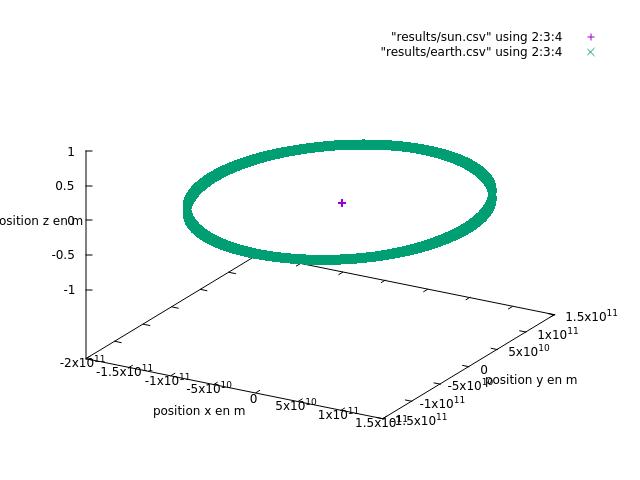
\includegraphics[width=1\linewidth]{modelisations/h=60s/positions-terre-soleil.png} 
\caption{h=84.6s}
\label{fig:1subim1}
\end{subfigure}
\begin{subfigure}{0.5\textwidth}
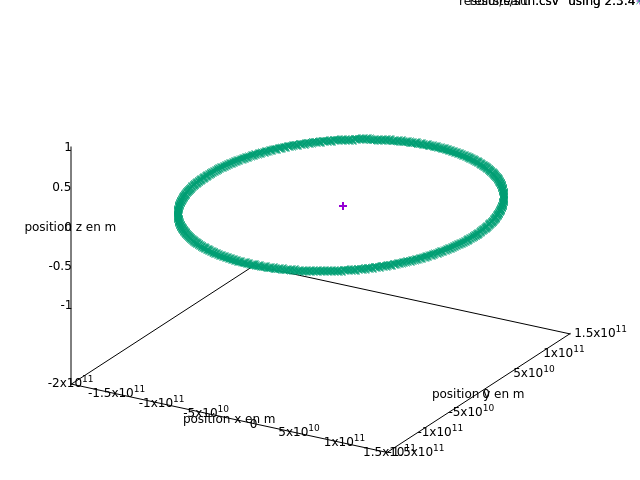
\includegraphics[width=1\linewidth]{modelisations/h=0.5j/positio_terre_sun_0.5.png}
\caption{h=1/2 j}
\label{fig:1subim2}
\end{subfigure}

\caption{Trajectoires de la Terre et du Soleil sur 2 avec RK4}
\label{fig:image2}
\end{figure}



Sur la figure \ref{fig:2subim1} on a tracé l'énergie total du système. On voit qu'elle oscille entre 1.3522e+34 J et 1.29996e+34 J, ce qui est normal puisque la distance entre la Terre et le soleil oscille, et donc la force exercé. Si on prend la moyenne on a 1.32608e+34 J, donc la variation est inférieur à 3\%\ on peut donc considéré notre énergie constante.

On note sur la figure \ref{fig:3subim1}, que l'aire parcours par la Terre reste constante au temps du temps à \(1.92463e+17 m^2\). La loi de Kepler est donc respecté.



\begin{figure}[H]
\begin{subfigure}{0.5\textwidth}
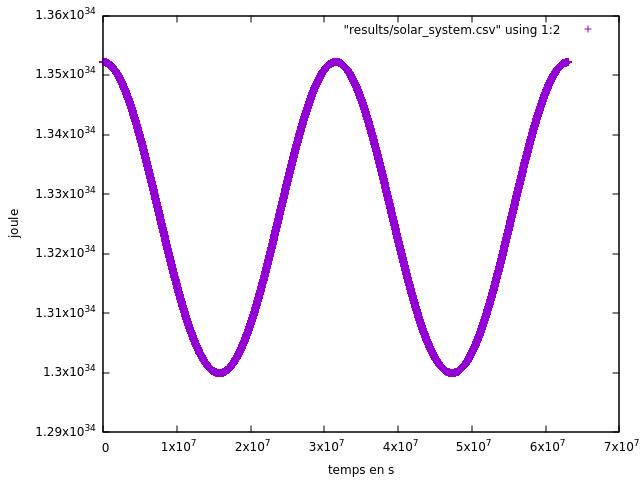
\includegraphics[width=1\linewidth]{modelisations/h=60s/energy_system.png}
\caption{h=84.6s}
\label{fig:2subim1}
\end{subfigure}
\begin{subfigure}{0.5\textwidth}
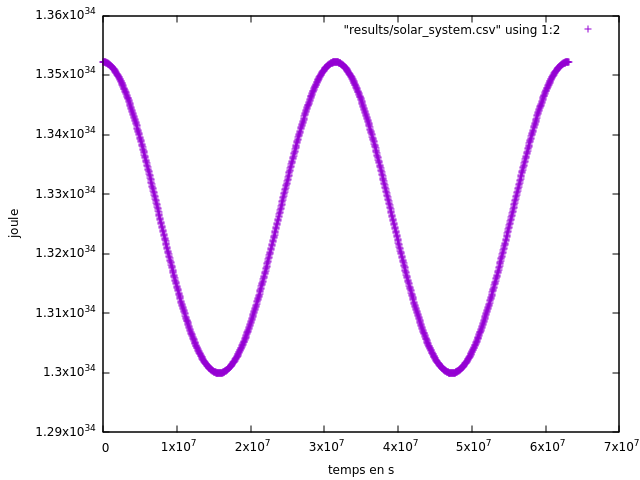
\includegraphics[width=1\linewidth]{modelisations/h=0.5j/energy_syst_0.5.png}
\caption{h=0.5 jours}
\label{fig:2subim2}
\end{subfigure}
\caption{Énergie totale du système sur 2 ans pour différents pas de temps, avec RK4}
\label{fig:image2}
\end{figure}

Pour la norme du moment cinétique de la Terre, visible sur la figure \ref{fig:4subim1}, on a un maximum à \(2.66139e+40 kg.m^2.s^1\) et un minimum à \(2.66123e+40 kg.m^2.s^1\). On trouve une moyenne de \(2.66131 e+40 kg.m^2.s^1\). Les variations sont en dessous des 2\%\ ce qui nous permet de conclure que le moment cinétique est constant au cours du temps pour la Terre.

Maintenant on a décidé de voir ce que donne l'aire \ref{fig:5subim1} et la norme du moment cinétique \ref{fig:5subim2} pour le Soleil. On remarque que pour le Soleil nous n'avons pas une aire ni un moment cinétique constant, mais on s'y attendait car ces informations sont principalement utiles pour les planètes.
\begin{figure}[H]
\begin{subfigure}{0.5\textwidth}
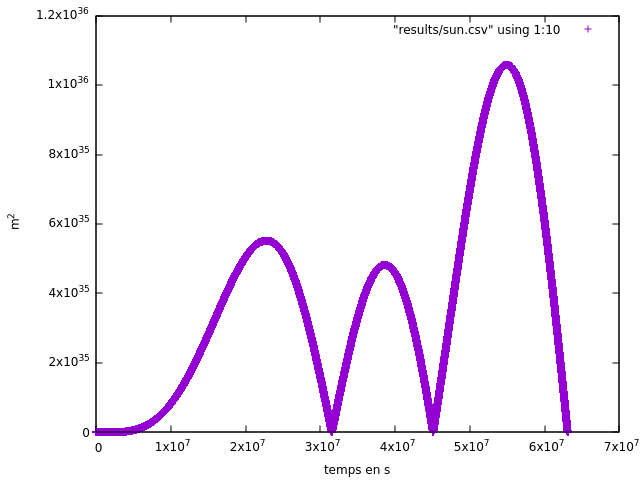
\includegraphics[width=1\linewidth]{modelisations/h=60s/aire-sun.png}
\caption{Aire Soleil}
\label{fig:5subim1}
\end{subfigure}
\begin{subfigure}{0.5\textwidth}
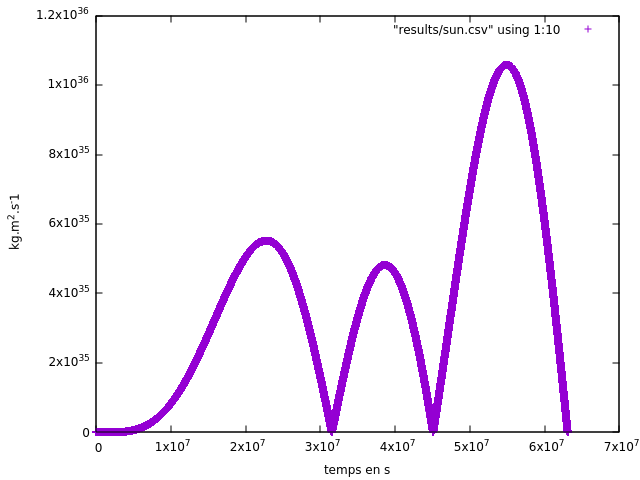
\includegraphics[width=1\linewidth]{modelisations/h=60s/mmc_sun.png}
\caption{Norme moment cinétique du Soleil}
\label{fig:5subim2}
\end{subfigure}
\caption{Norme du moment cinétique et Aire du Soleil pour h=84.6s}
\label{fig:image2}
\end{figure}


\subsubsection{h=0.5*24*3600 donc pour 1/2 journée}
On  simule cette fois pour h=1/2 j, la simulation s'est faite en moins de 1s. Le pas de temps étant plus grand, le temps de calcul est beaucoup plus court. Sur \ref{fig:1subim2} on a la même trajectoire du système (Terre/Soleil) pour h=1/2 j que pour 84.6s. Pour ce pas de temps on a encore de bonnes trajectoires.

Sur la figure \ref{fig:2subim2} on a tracé l'énergie total du système. On voit qu'elle oscille entre 1.3522e+34 J et 1.29996e+34 J, ce qui est normale puisque la distance entre la Terre et le soleil oscille, et donc la force exercé. Si on prend la moyenne on a 1.32608e+34 J, donc la variation est inférieur à 3\%\ on peut donc considéré notre énergie constante. 


On note sur la figure \ref{fig:3subim2}, que l'aire parcours par la Terre reste constante au temps du temps à \(1.92459e+20 m^2\). La loi de Kepler est donc respecté. On remarque qu'on a pas la même valeur qu'avec h=84.6s.

Pour la norme du moment cinétique de la Terre, visible sur la figure \ref{fig:4subim2}, on a un maximum à \(2.66139e+40 kg.m^2.s^1\) et un minimum à \(2.66123e+40 kg.m^2.s^1\). Une trouve une moyenne de \(2.66131 e+40 kg.m^2.s^1\). Les variations sont en dessous des 2\%\ ce qui nous permet de conclure que le moment cinétique est constant au cours du temps pour la Terre.


\subsubsection{h=24*3600 1 jour}
On  simule pour un dernier pas de temps h=1 j, la simulation c'est faite en moins de 1s. On a la trajectoire du système (Terre/Soleil) pour tous les pas de temps (graphiquement on ne voit aucune différence). Pour ce pas de temps on a encore de bonnes trajectoires. 

Pour l'énergie totale, on observe la même chose que pour les précédents pas de temps.

On note sur la figure \ref{fig:3subim3}, que l'aire parcours par la Terre reste constante au temps du temps à \(9.62302e+19 m^2\). La loi de Kepler est donc respecté. On remarque qu'on a pas la même valeur qu'avec h=84.6s, et h=1/2 j.

Pour la norme du moment cinétique de la Terre, visible sur la figure \ref{fig:4subim3}, on a un maximum à \(2.66139e+40 kg.m^2.s^1\) et un minimum à \(2.66123e+40 kg.m^2.s^1\). Une trouve une moyenne de \(2.66131 e+40 kg.m^2.s^1\). Les variations sont en dessous des 2\%\ ce qui nous permet de conclure que le moment cinétique est constant au cours du temps pour la Terre.

Pour conclure sur le test des pas de temps, on peut voir que globalement le pas de temps ne change pas les résultats, sauf pour l'aire parcourue par la Terre qui diminue quand le pas de temps augmente, donc quand la précision diminue. Si on avait fais ce test avec une fonction de résolution moins précise comme Euler, on aurait peut-être eu plus de disparité entre les pas de temps.


\begin{figure}[H]
\begin{subfigure}{0.5\textwidth}
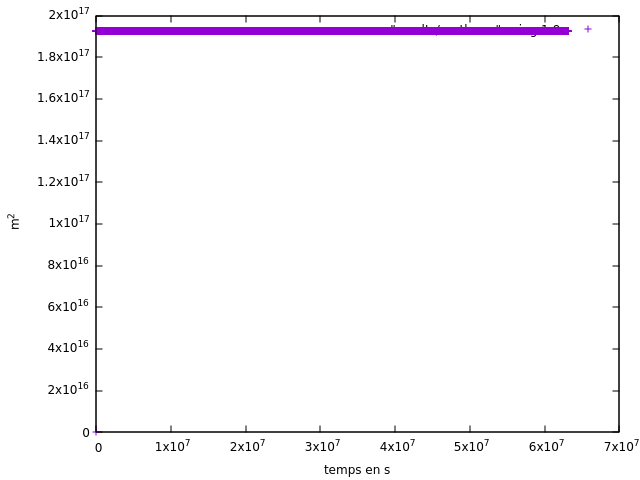
\includegraphics[width=1\linewidth]{modelisations/h=60s/aire_terre.png}
\caption{h=84.6s Aire Terre}
\label{fig:3subim1}
\end{subfigure}
\begin{subfigure}{0.5\textwidth}
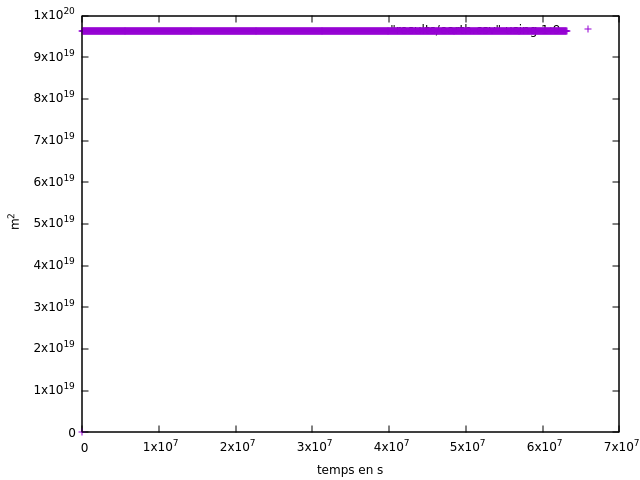
\includegraphics[width=1\linewidth]{modelisations/h=0.5j/aire_terre_0.5.png}
\caption{h=0.5 jours Aire Terre}
\label{fig:3subim2}
\end{subfigure}
\begin{subfigure}{0.5\textwidth}
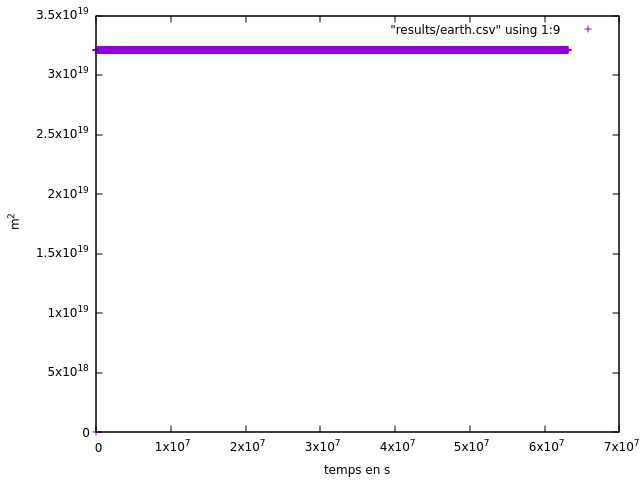
\includegraphics[width=1\linewidth]{modelisations/h=j/aire_terre_1.png}
\caption{h=1 jour Aire Terre}
\label{fig:3subim3}
\end{subfigure}
\begin{subfigure}{0.5\textwidth}
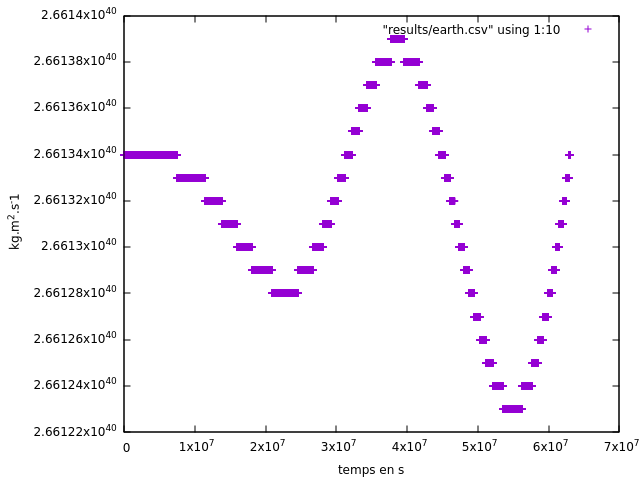
\includegraphics[width=1\linewidth]{modelisations/h=60s/mmc_terre.png}
\caption{h=84.6s Moment cinétique de la Terre}
\label{fig:4subim1}
\end{subfigure}
\begin{subfigure}{0.5\textwidth}
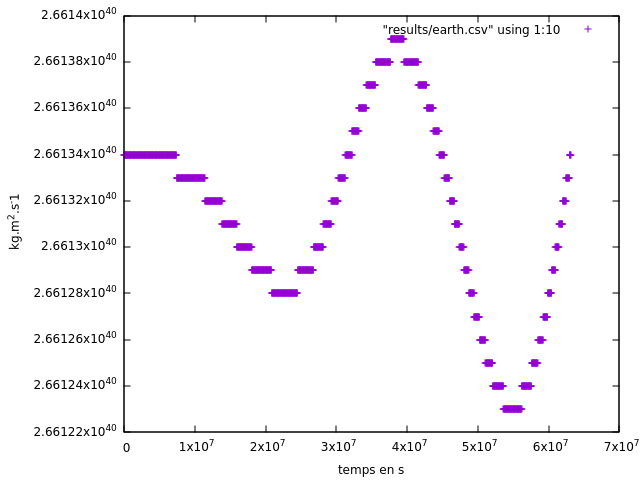
\includegraphics[width=1\linewidth]{modelisations/h=0.5j/mmc_earth_0.5.png}
\caption{h=0.5 jours Moment cinétique de la Terre}
\label{fig:4subim2}
\end{subfigure}
\begin{subfigure}{0.5\textwidth}
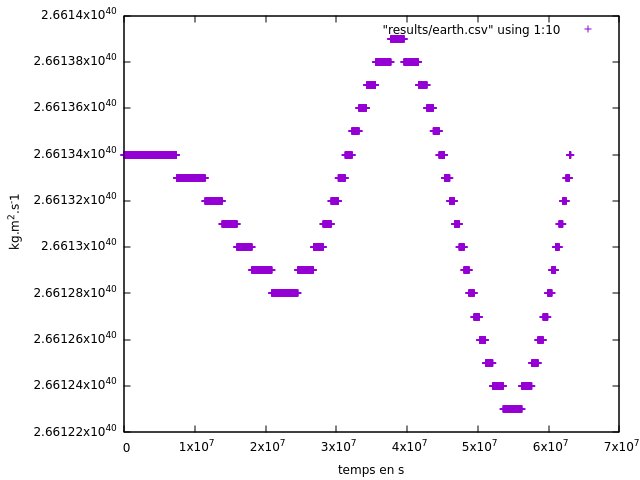
\includegraphics[width=1\linewidth]{modelisations/h=j/mmc_terre_1.png}
\caption{h=1 jour Moment cinétique de la Terre}
\label{fig:4subim3}
\end{subfigure}
\caption{Moment cinétique de la Terre et son aire sur 2 ans pour différents pas de temps, avec RK4}
\label{fig:image2}
\end{figure}
\subsection{Test des fonctions de résolution}
Nous avons testé pour un même pas de temps, ici h=1/2 journée, et comparer rk4, Verlet et Euler. Le but est de savoir si une des méthodes ce démarque des autres.

\begin{figure}[H]
\begin{subfigure}{0.5\textwidth}
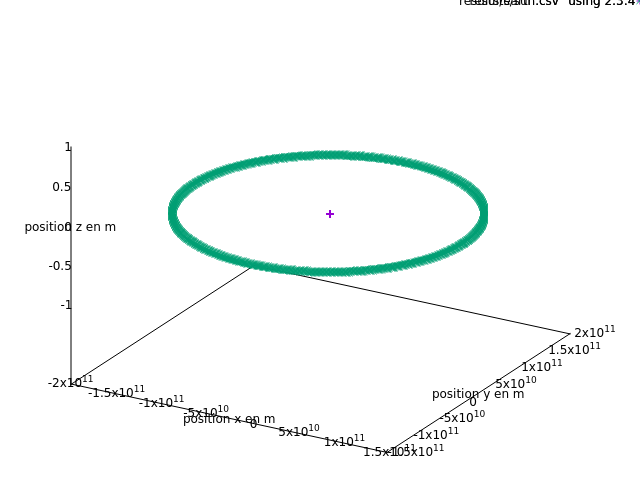
\includegraphics[width=1\linewidth]{eulerverlet/positions_terre_soleil_verlet.png}
\caption{Verlet}
\label{fig:6subim1}
\end{subfigure}
\begin{subfigure}{0.5\textwidth}
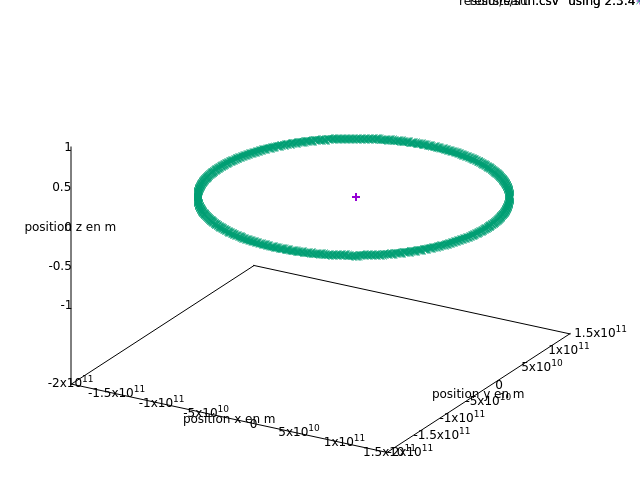
\includegraphics[width=1\linewidth]{eulerverlet/positions_terre_soleil_euler.png}
\caption{Euler}
\label{fig:6subim2}
\end{subfigure}

\caption{Trajectoire de la Terre et du Soleil pour une demi journée de pas de temps avec Verlet et Euler}
\label{fig:image2}
\end{figure}

\begin{figure}[H]
\begin{subfigure}{0.5\textwidth}
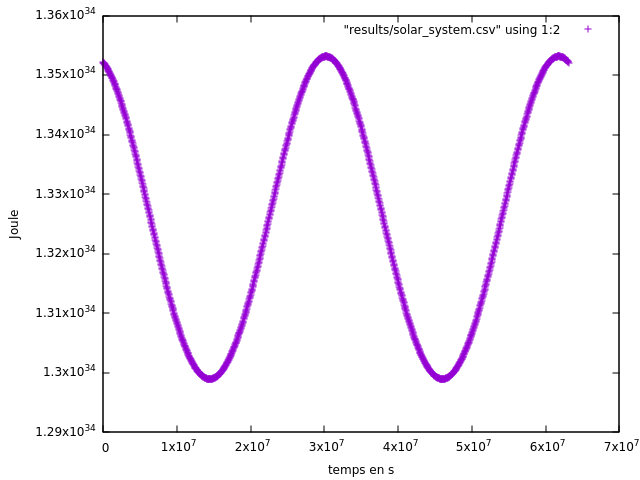
\includegraphics[width=1\linewidth]{eulerverlet/energy_sol_syst_verlet.png}
\caption{Verlet}
\label{fig:7subim1}
\end{subfigure}
\begin{subfigure}{0.5\textwidth}
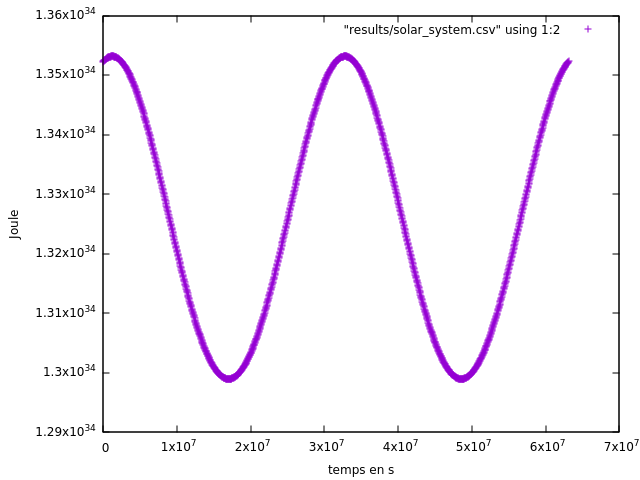
\includegraphics[width=1\linewidth]{eulerverlet/energy_sol_syst_euler.png}
\caption{Euler}
\label{fig:7subim2}
\end{subfigure}

\caption{Énergie totale du système pour une demi journée de pas de temps avec Verlet et Euler}
\label{fig:image2}
\end{figure}

On a les résultats de rk4 dans la partie précédente pour h=1/2 journée, on passe donc directement à Euler. Pour ce pas de temps et cette méthode, les calculs se font en moins d'une minute. On trouve une énergie totale \ref{fig:7subim1} maximal à 1.35315e+34 J et minimal à 1.29897e+34 J. On calcule la moyenne à 1,32606e+34 J, on a comme avec RK4 une différence inférieur à 3\%\. 
L'aire parcouru par la Terre \ref{fig:8subim1} est de \(9.62305e+19 m^2\), plus faible que le résultat obtenue avec rk4 pour le même pas de temps mais qui ce rapport de rk4 à h=1 j. Pour la norme du moment cinétique Terre on a au maximum 2.66139e+40 \(kg.m^2.s^1\) \ref{fig:9subim1}, et au minimum 2.66123e+40 \(kg.m^2.s^1\). On a en moyenne 2,66131e+40, soit moins de 2\%\ de différence.

\begin{figure}[H]
\begin{subfigure}{0.5\textwidth}
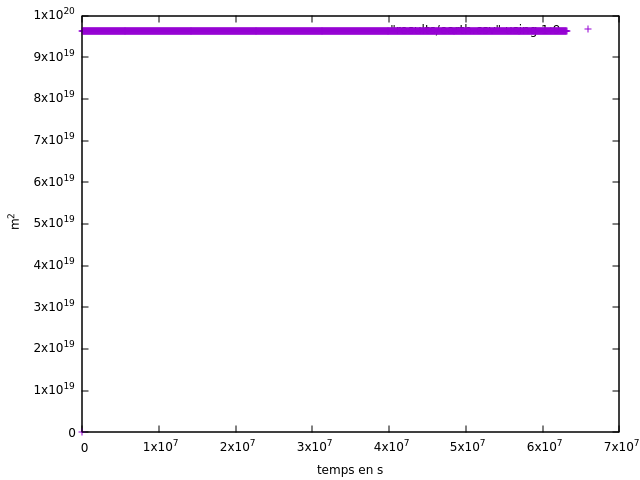
\includegraphics[width=1\linewidth]{eulerverlet/aire_terre_verlet.png}
\caption{Verlet}
\label{fig:8subim1}
\end{subfigure}
\begin{subfigure}{0.5\textwidth}
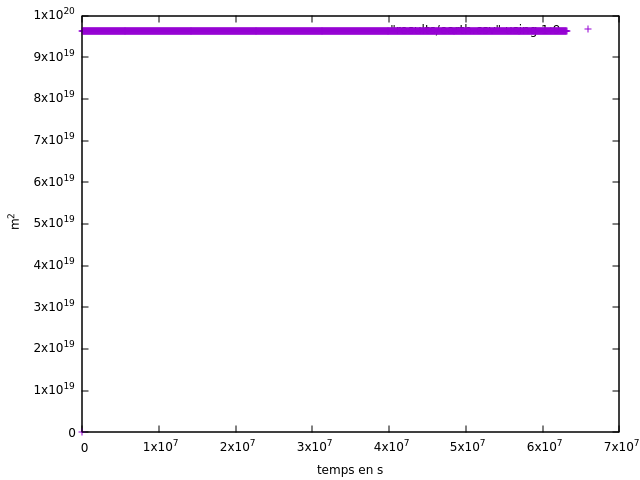
\includegraphics[width=1\linewidth]{eulerverlet/aire_terre_euler.png}
\caption{Euler}
\label{fig:8subim2}
\end{subfigure}

\caption{Aire de la Terre pour une demi journée de pas de temps avec Verlet et Euler}
\label{fig:image2}
\end{figure}

\begin{figure}[H]
\begin{subfigure}{0.5\textwidth}
\includegraphics[width=1\linewidth]{eulerverlet/moment_cinét_terre_verlet.png}
\caption{Verlet}
\label{fig:9subim1}
\end{subfigure}
\begin{subfigure}{0.5\textwidth}
\includegraphics[width=1\linewidth]{eulerverlet/moment_cinét_terre_euler.png}
\caption{Euler}
\label{fig:9subim2}
\end{subfigure}

\caption{Norme du moment cinétique de la Terre pour une demi journée de pas de temps avec Verlet et Euler}
\label{fig:image2}
\end{figure}

On remarque qu'on a graphiquement aucune différence visible au niveau des trajectoire pour rk4 \ref{fig:1subim1}, Verlet \ref{fig:6subim1}, et Euler \ref{fig:6subim2}.



Avec Verlet l'énergie totale \ref{fig:7subim2} maximal 1.35216e+34 J, et au minimum 1.29897e+34 J. En moyenne on 1,325565e+34 J, moins de 3\%\ comme avec RK4 et Euler. 
L'aire parcouru par la Terre \ref{fig:8subim2} est de \(9.62278e+19 m^2\), plus faible que le résultat obtenue avec rk4 et Verlet pour le même pas de temps. Pour la norme du moment cinétique Terre on a au maximum 2.66139e+40 \(kg.m^2.s^1\) \ref{fig:9subim2}, et au minimum 2.66123e+40 \(kg.m^2.s^1\). On a en moyenne 2,66131e+40, soit moins de 2\%\ de différence comme avec Verlet et rk4.
\\[2 mm]
On a donc une différence visible au niveau de l'aire de la Terre calculé par les différentes méthodes, mais pas de façon significative puisqu'on reste dans le même ordre de grandeur.

\subsection{Modélisation du système sur 43ans avec un pas de temps de 60s}

Nous avons voulu après les tests nécessaires pour assurer le fonctionnement de notre programme, lancer une simulation de plus grande ampleur. Nous avons simulé l'orbite de toutes les planètes autour du soleil sur 90 ans avec un pas de 60s. Nous tenons à signaler que la simulation devait prendre quasiment 5 jours celle-ci s'est arrêtée suite à une coupure électrique au bout de 3 jours ce qui fait que nous avons eu seulement 43 ans de simulation.

\begin{figure}[H]
\begin{subfigure}{0.5\textwidth}
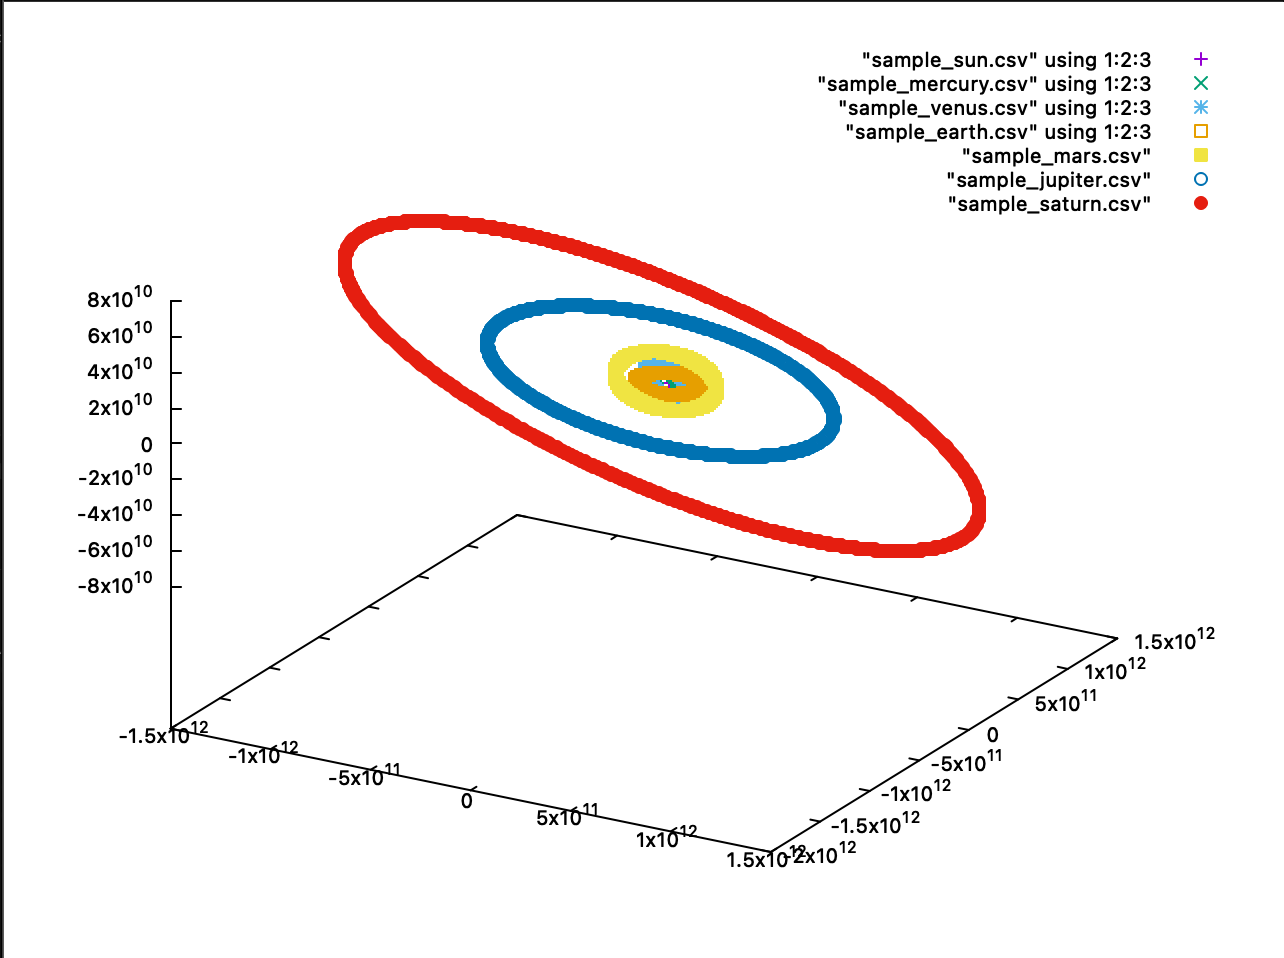
\includegraphics[width=1\linewidth]{43y.png} 
\caption{Trajectoire des planètes de Mercure jusqu'à Saturne, avec le Soleil, sur 43ans et un pas de temps de 60s}
\label{fig:asubim1}
\end{subfigure}
\begin{subfigure}{0.5\textwidth}
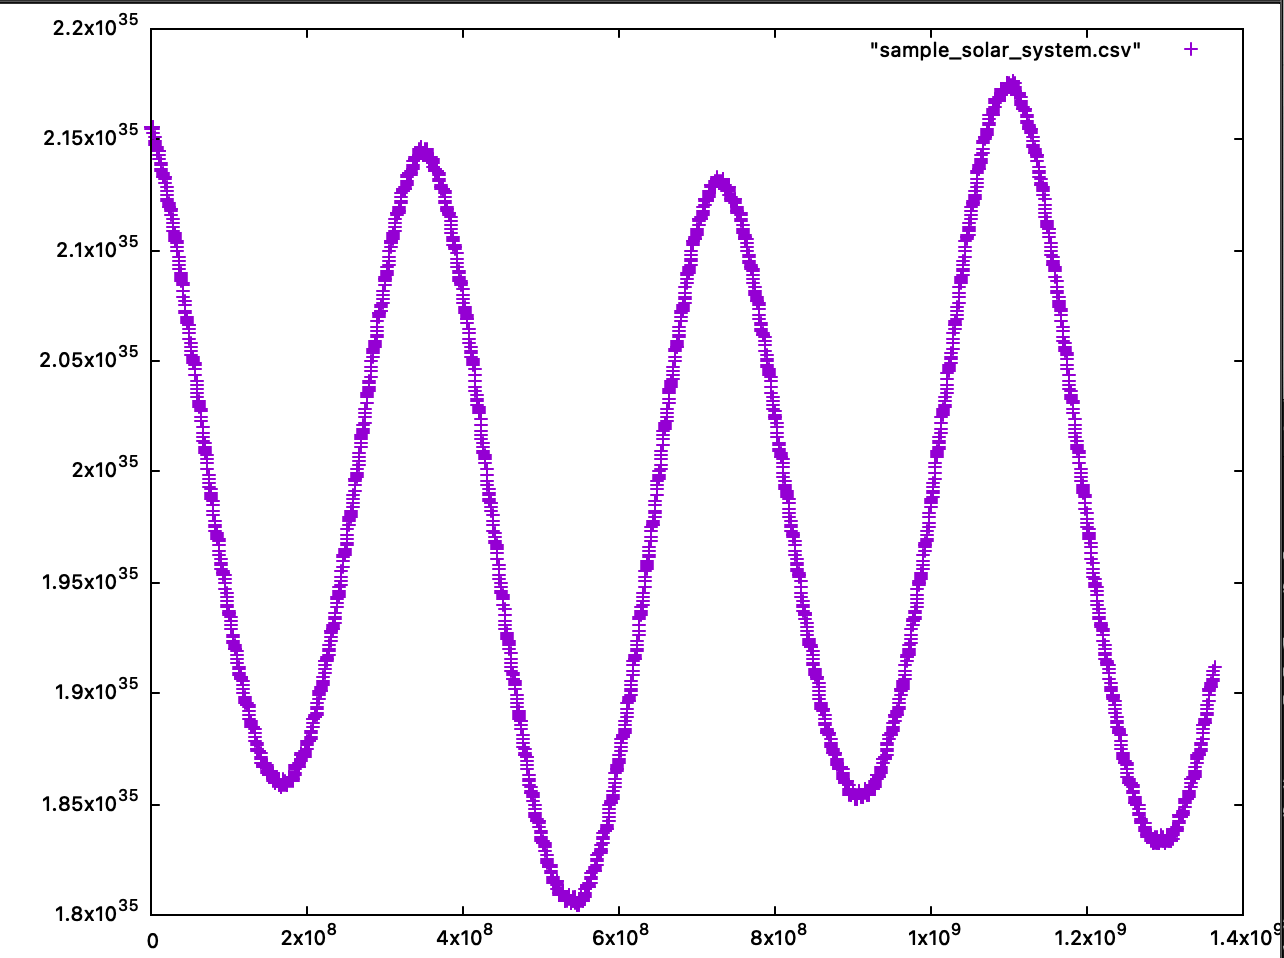
\includegraphics[width=1\linewidth]{43y tot energy.png}
\caption{Énergie totale du système en J et en fonction du temps}
\label{fig:bsubim2}
\end{subfigure}
\begin{subfigure}{0.5\textwidth}
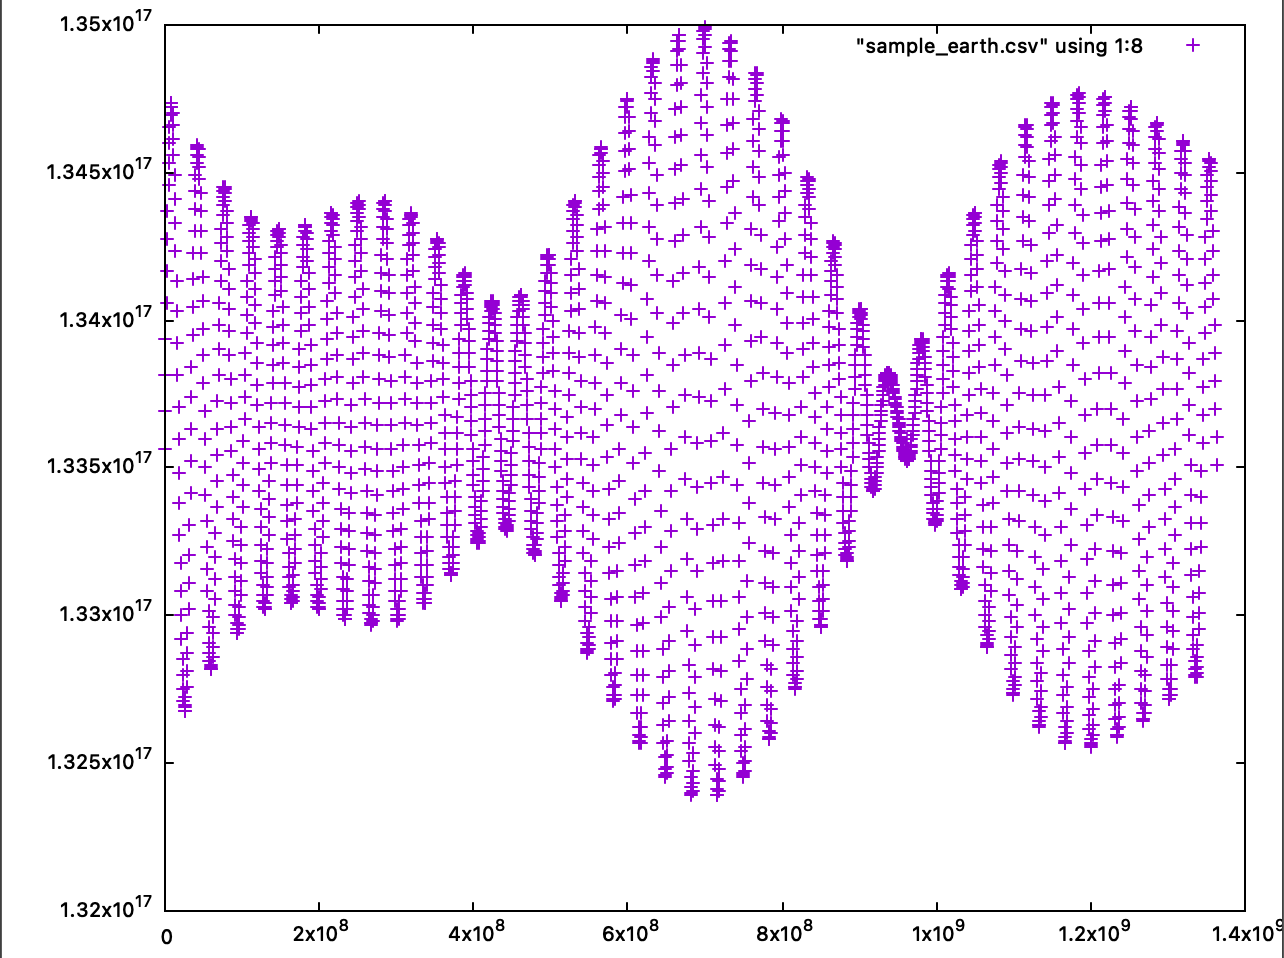
\includegraphics[width=1\linewidth]{43y area earth.png}
\caption{Aire de la Terre en \(m^2\) et en fonction du temps}
\label{fig:csubim3}
\end{subfigure}
\begin{subfigure}{0.5\textwidth}
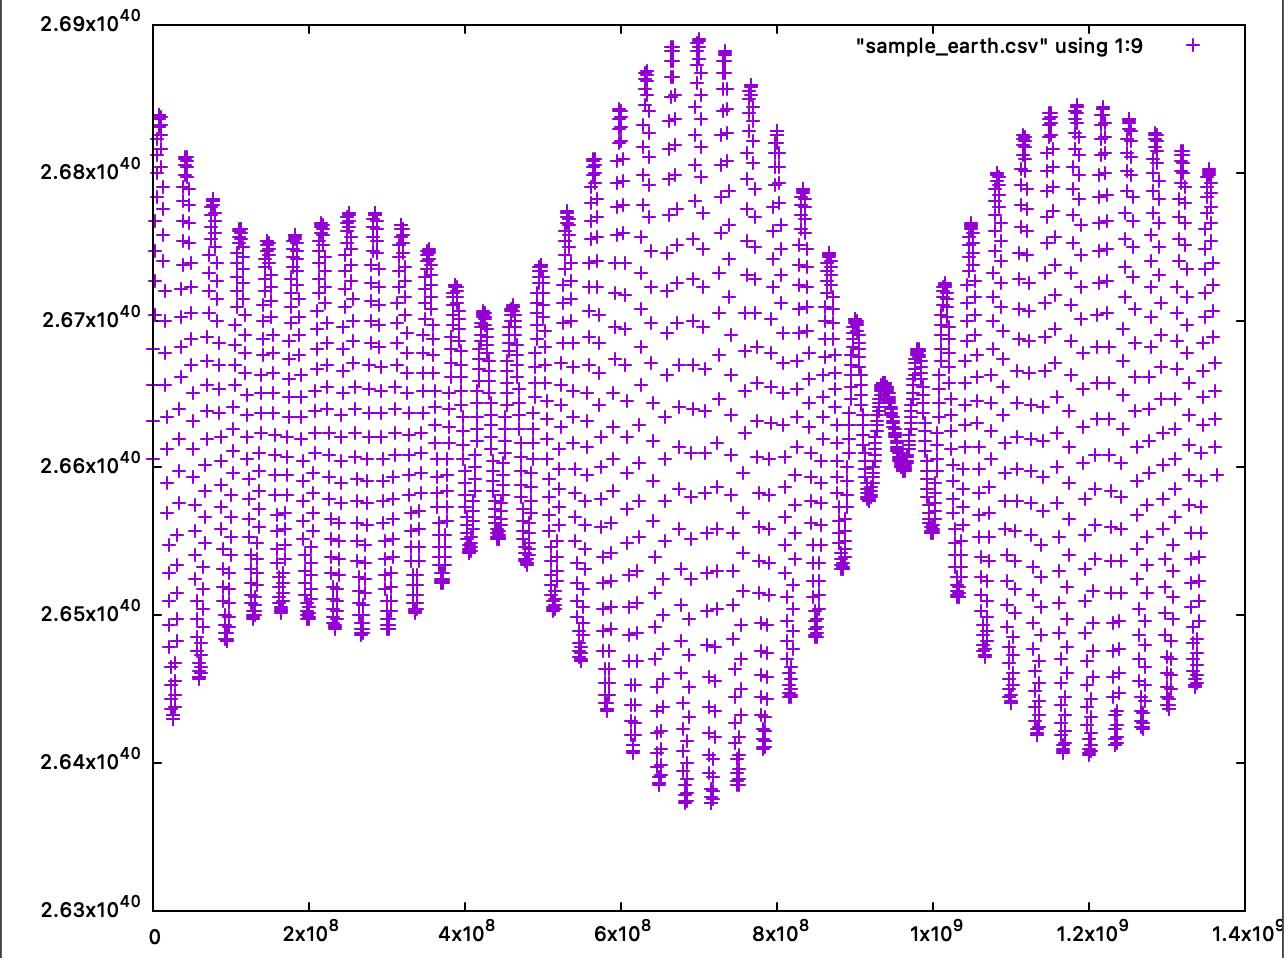
\includegraphics[width=1\linewidth]{43y cinematic moment earth.png}
\caption{Moment cinétique de la Terre}
\label{fig:dsubim4}
\end{subfigure}
\caption{Modélisation du système sur 43ans avec un pas de temps de 60s}
\label{fig:image2}
\end{figure}

Le premier graphique \ref{fig:asubim1} nous présente les orbites des planètes (les plus petites sont peu distinguables). Nous voyons, conformément à nos attentes que les orbites des planètes sont extrêmement précises avec ce petit pas de temps.

Le deuxième graphique \ref{fig:bsubim2}, nous renseigne sur l'énergie totale du système solaire.  Cette dernière oscille autour d'un point et on peut voir une conservation en moyenne de l'énergie totale. On sait que la masse du système solaire est contenue dans le soleil en grande partie et que l'on devrait trouver dans le cas de cette simulation précise une énergie d'environ 
$E = 10^{35} J$. Le graphique montre bien qu'on se situe dans l'ordre de grandeur attendu.

Ensuite, nous avons pris le partie d'étudier les grandeurs caractéristiques de l'orbite de la terre pour vérifier le comportement d'une planète et de surtout pouvoir comparer ce comportement avec les autres planètes. Sur le graphique \ref{fig:csubim3}, on peut voir l'évolution de l'aire parcourue par la Terre et on voit ici apparaître des oscillations. On remarque très vite que ces oscillations sont dues à la présence des autres planètes dans ce système. Le moment cinétique présenté dans la figure \ref{fig:dsubim4}, nous fait remarquer la même chose.



\section{Problèmes rencontrés}

La mise en équation nous a posé problème parfois notamment lors du moment où nous avons commencé le développement des fonctionnalités associées à RK4. Plusieurs problèmes ont émergé autour de la structure que nous avons voulu donner au programme dans son ensemble notamment avec une multitude de réfaction. Le diagramme UML que nous avons présenté nous a largement permis de progresser rapidement surtout pour comprendre et nous rappeler comment sont instanciés les classes entre elles.

Lorsque nous avons commencé à développer Verlet nous avons eu un énorme problème de stabilité, ceci venait du fait que nous forcions le soleil au centre alors que nous nous devions d'utiliser un système de coordonnées centré dans le barycentre des masses du système. Sans cette compréhension, à chaque pas de temps nous éloignons les planètes du soleil ce qui aboutissait à des divergences.

Le versionnage avec Github nous a permis d'aborder une manière de programmer plus professionnelle et organisée. Effectivement en versionnant notre programme à chaque fois que nous développions une fonctionnalité qui était soit inutile soit vouée à un échec nous pouvions revenir à des versions précédentes et fonctionnelles très facilement.

Lorsque nous avons commencé les problèmes à N corps nous avons voulu simuler des systèmes avec des objets légers et/ou éloignés tels que des astéroïdes ou des planètes naines. Ces simulations se sont soldées par des échecs car les forces en jeu étaient plus petites que le 0 machine donc nous avons abouti à de fortes divergences du calcul avec notamment des divisions par 0.

\section{Conclusion}
Nous avons choisi de prendre un projet qui nous intéressait énormément à tous les deux, la compréhension des équations et leurs intégrations n'étaient pas très compliquées cependant nous avons choisi de développer le programme en programmation orientée objet pour avoir une structure rapidement évolutive et intelligible pour le lecteur. En plus de cette orientation de programmation, le projet a été écrit sous la forme d'une API pour réaliser rapidement des calculs et pour pouvoir ajouter facilement des objets.

L'apprentissage de la commande git et des spécificités du versionnage  en collaboration (merging, fetching...) a pris beaucoup de temps mais cet investissement est excellent pour travailler efficacement sur ce projet ou pour la suite de nos études/carrières

De plus, il était très gratifiant de voir des résultats arriver rapidement et de pouvoir analyser les défauts qui persistaient dans notre programme pour pouvoir rapidement les corriger. Le programme a plusieurs fois posé des problèmes de sémantiques et nous a obligé de réfléchir à des structures différentes. Il était très intéressants de s'obliger de se poser quelques heures afin de discuter des orientations que l'on allait prendre sans écrire une seule ligne en réfléchissant seulement à un programme simple pour le lecteur et l'utilisateur.

Enfin, comme nous l'avons vu ce programme est basé sur des calculs de forces d'interactions afin de calculer de nouvelles positions et vitesses, ici nous avons utilisé la force gravitationnelle pour modéliser des systèmes planétaires mais rien n'empêche de faire évoluer ce programme pour ajouter de nouvelles forces d'interactions (coulomb, interaction faible...) et arriver à modéliser de nouveaux systèmes en interactions (particules, atomes, molécules...). 

\section{Bibliographie}
https://prappleizer.github.io/#tutorials\\
Programmer en C++ moderne, De Claude Delannoy\\
Tosun, Buğra. (2020). Computation of Satellite Orbits by Using Numerical Methods. \\

\end{document}